\documentclass[11pt]{article}
\usepackage{geometry}
\geometry{a4paper, left=25mm, right=25mm, top=25mm, bottom=30mm}

\usepackage{amsmath}
\usepackage{graphicx}
\usepackage{booktabs}
\usepackage{siunitx}
\usepackage{microtype}
\usepackage{parskip}
\usepackage{hyperref}
\usepackage{xcolor}
\usepackage{listings}
\usepackage{titling}
\usepackage{mdframed}
\usepackage{changepage}

\definecolor{codegreen}{rgb}{0.33, 0.71, 0.36}
\definecolor{codegray}{rgb}{0.5, 0.5, 0.5}
\definecolor{codepurple}{rgb}{0.58, 0, 0.82}
\definecolor{backcolour}{rgb}{0.95, 0.95, 0.92}
\definecolor{codeblue}{rgb}{0.25,0.5,0.8}

\lstset{
    backgroundcolor=\color{backcolour},   
    commentstyle=\color{codegreen},
    keywordstyle=\color{codeblue},
    numberstyle=\tiny\color{codegray},
    stringstyle=\color{codepurple},
    basicstyle=\ttfamily\footnotesize,
    breakatwhitespace=false,         
    breaklines=true,                 
    captionpos=b,                    
    keepspaces=true,                 
    numbers=left,                    
    numbersep=5pt,                  
    showspaces=false,                
    showstringspaces=false,
    showtabs=false,                  
    tabsize=2,
    language=Python
}

\title{}
\author{Sebastian M.D.}
\date{March 2024}

\mdfdefinestyle{leftLine}{
    linecolor=black,
    outerlinewidth=1pt,
    bottomline=false,
    topline=false,
    rightline=false,
    leftmargin=10pt,
    rightmargin=10pt,
    skipabove=0pt,
    skipbelow=0pt,
    innertopmargin=0pt,
    innerbottommargin=0pt,
}

\pretitle{%
  \begin{center}
  \begin{mdframed}[style=leftLine]
    Supervisor: Thomas Lennartson
    
    Program: Natural Sciences Program
    
    School: Procivitas Privata Gymnasium Malmö 
    \end{mdframed} 
    \vspace{3em}
  \huge
Which Neural Network Architecture is Optimal for Predicting Chaotic Dynamics? \\
\vspace{1em}
\small
\begin{adjustwidth}{2cm}{2cm}
A comparative study between RNN, Transformers and Echo State Networks regarding their capacity to predict the Lorenz 63 system.
\end{adjustwidth}
\vspace{14em}
\begin{figure}[h]
\centering
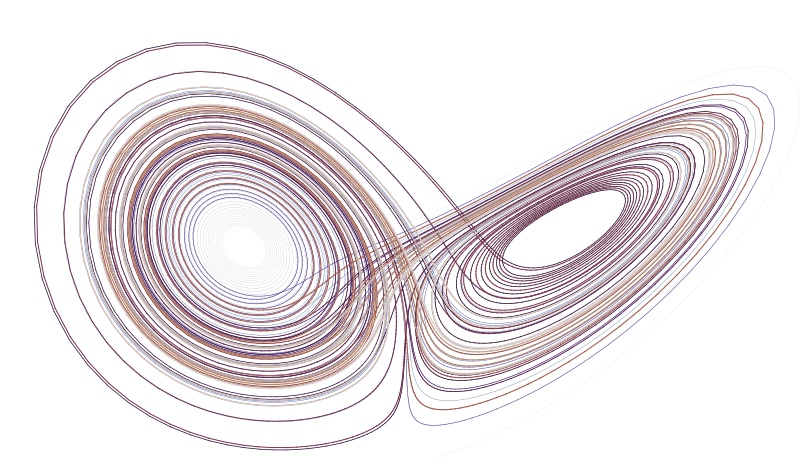
\includegraphics[width=0.8\textwidth]{title_page_image.jpeg}
\end{figure}

}
\posttitle{\end{center}}



\preauthor{\vfill\begin{center}\large}
\postauthor{\end{center}}

\predate{\begin{center}\large}
\postdate{\end{center}}

\begin{document}


\maketitle
\thispagestyle{empty} % Removes the page number

\newpage
\null\vspace*{\stretch{1}}
\begin{abstract}
    % Should be complete overview of purpose, method, results and conclusion, needs to be rewritten
\noindent This paper explores the application of neural networks in predicting the trajectory of the Lorenz 63 system, a set of differential equations that showcase chaotic behavior. The Lorenz System was originally stipulated by Edward N. Lorenz in 1963 as a mathematical model for atmospheric convection and is commonly used as a toy problem to explore chaos theory. Traditional numerical methods such as the Runga Kutta 4th order method can be used to solve and predict the system's behavior. This study explores the use of neural networks as an alternative approach to predict chaos. The methodology involves training a neural network on a dataset generated from the Lorenz system via the RK4 method. By using a small step size and high computational resources, the network can generalize patterns and possibly later on efficiently predict the system's future state with different initial conditions. This paper aims to test the RNN LSTM, Transformers, and RC-ESN network architectures. RNN and Transformer architectures are known for their ability to handle sequential data, while RC-ESN is known for its ability to capture chaotic systems. The results of the study will be compared to the RK4 method to determine if the neural networks could surpass it with a greater prediction horizon given similar computational resources.
\end{abstract}
\vspace*{\stretch{2}}
\newpage


\tableofcontents
\newpage

\section{Introduction}
A chaotic system is a dynamical system that is highly sensitive to initial conditions, leading to long-term unpredictability despite its deterministic nature. Chaotic systems are found in many natural phenomena, such as weather, water flows, and planetary orbits. Traditionally chaotic systems have been modeled using numerical methods, however papers such as \cite{npg-27-373-2020} have tried to apply neural network models instead. Neural networks are computing systems that mimic the brain to learn from data and recognize patterns without explicit instructions. Results have shown that neural networks, specifically echo state networks, can be promising in capturing chaotic dynamics. The goal of this study is to further explore the application of neural networks by also testing out the Transformers architecture as introduced by Google in their research paper \cite{DBLP:journals/corr/VaswaniSPUJGKP17} and compare it to the RNN and ESN architectures. The networks will be judged on their mean squared error over time and their ability to capture the Lorenz 63 system's chaotic patterns. The objective is to detemine which of these architecture prove most effective in predicting chaotic systems.
\section{Theory}

\subsection{The Lorenz System}

The original Lorenz system is a set of three differential equations. It is one of the earliest and most studied examples of systems that exhibit chaotic behavior. It is defined by the following equations:

\begin{align}
\frac{dx}{dt} &= \sigma(y - x) \\
\frac{dy}{dt} &= x(\rho - z) - y \\
\frac{dz}{dt} &= xy - \beta z
\end{align}

where $x$, $y$, and $z$ make up the system's positional state with respect to time $t$, and $\sigma$, $\rho$, and $\beta$ are parameters. Typically, the values $\sigma = 10$, $\rho = 28$, and $\beta = \frac{8}{3}$ are used.

The Lorenz system is known for its butterfly-shaped attractor, which is a set of points the system, regardless of the starting condition, always end up at. The attractor is visualized in Figure \ref{fig:lorenz_attractor}.

\begin{figure}[h]
\centering
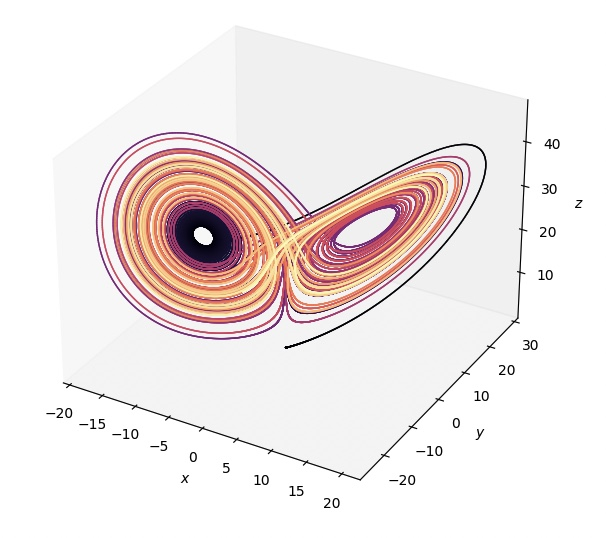
\includegraphics[width=0.3\textwidth]{lorenz_attractor.jpeg}
\caption{The Lorenz attractor for $\sigma = 10$, $\rho = 28$, and $\beta = \frac{8}{3}$. Generated with RK4 method for 100 time units}
\label{fig:lorenz_attractor}
\end{figure}

\subsection{Neural Networks}

Neural networks are a type of machine learning model that are inspired by the structure of the human brain. They are composed of layers with interconnected nodes, which represent neurons, that process input data and produce an output. These nodes are usually connected to each other with linear transformations called weights (\(W\)) and biases (\(b\)). The weights and biases are the parameters of the network that initially are randomly initialized and are optimized during the training process. \\

At the heart of neural networks is the feedforward computation that passes the data from one layer \(x\) to the next \(y\) as follows:

\[ y = f(Wx + b) \]

where \(y\) is the output, \(W\) is the weights matrix, \(x\) is the input vector, \(b\) is the bias vector, and \(f\) is the activation function, typically the ReLU(rectified linear unit) function is used. the ReLU function is defined as:

\[ \text{ReLU}(z) = \max(0, z) \]

Which maps all positive inputs to themselves while negative inputs are mapped to zero. The ReLU activation function introduces non-linearity to the model, which is critical for capturing complex behavior. Another popular activation function is the hyperbolic tangent or tanh, which squashes the input values to be within the range \(-1\) and \(1\):

\[
\text{tanh}(z) = \frac{e^{z} - e^{-z}}{e^{z} + e^{-z}}
\]

This allows tanh to output values that have mean zero, which can make learning for the subsequent layers slightly easier. Another activation function commonly used for the output layer is the sigmoid function. The sigmoid function maps the input values to a range between \(0\) and \(1\), interpreted as probabilities:

\[
\sigma(z) = \frac{1}{1 + e^{-z}}
\]

Due to its shape, the sigmoid function is suitable for binary outputs and is useful when a probabilistic interpretation is desired for the output neuron. However, for multiclass classification tasks, the softmax activation function is commonly used instead. It maps the input vector to a probability distribution:

\[
\text{softmax}(z_i) = \frac{e^{z_i}}{\sum_{j=1}^{K} e^{z_j}}
\]

The softmax function ensures that the sum of the probabilities of all classes is \(1\), which is great for a probabilistic interpretation.

Given a predicted value \(\hat{y}_i\) and a true value \(y_i\) a cost function is used to measure the degree of error in the prediction. Commonly used for regression-based tasks is the mean squared error (MSE) function, which is defined by:

\[ C = \frac{1}{2n} \sum_{i=1}^{n} (y_i - \hat{y}_i)^2 \]

where \(C\) is the cost, \(n\) is the number of samples, \(y_i\) is the true value, and \(\hat{y}_i\) is the predicted value.

During the training process, optimization strategies such as stochastic gradient descent (SGD) are used. The gradient of the cost function is computed with respect to the weights in a process called backpropagation, and is used to adjust the weights in the direction that minimizes the cost:

\[ W_{\text{new}} = W_{\text{old}} - \eta \nabla C \]

where \(W_{\text{new}}\) and \(W_{\text{old}}\) are the values of the weights after and before the update, respectively, \(\nabla C\) is the gradient of the cost function with respect to the weights, and \(\eta\) is the learning rate.

Via processes like SGD, the network can compute a gradient to slowly shift the parameters and minimize the error of the network's predictions. Over time the network can generalize and learn the underlying patterns of the data to make accurate predictions on unseen data.

\subsection{RNNs}
A Recurrent Neural Network (RNN) is a type of neural network architecture designed to recognize patterns in sequential data. What makes the RNN architecture special is that it's composed of a train of nodes, called cells, each connected to the next, where all the cells share the same trainable weights and biases. Each node in the train has it's own hidden state that is used when computing the next ouput. When the input vector is fed to the first cell of the train, it creates an output and then the hidden state is updated and passed along to the next node. The hidden state makes it so the next cell can 'remember' the previous data inputed. The RNN is governed by these equations:

\begin{equation}
h^{(t)} = \tanh(Wh^{(t-1)} + Ux^{(t)} + b_h)
\end{equation}

\begin{equation}
y^{(t)} = \text{softmax}(Vh^{(t)} + b_y)
\end{equation}

Here \(h^{(t)}\) is the hiddens state at timestep $t$, and \(y^{(t)}\) the equivalent output at that timestep. The weights $W$, $U$ and $V$ and the biases $b_h$ and $b_y$ are trainable parameters of the network and they are the same for all nodes. These equations highlight the recurrent nature of the RNN, as the computation of the hidden state at time $t$ depends on the previous state at $t-1$. This is what allows the network to maintain a form of memory over time. See Figure 2 for a visual representation of the RNN architecture, where $o^{(t)}$ represents $y^{(t)}$ before softmax

\begin{figure}[h]
\centering
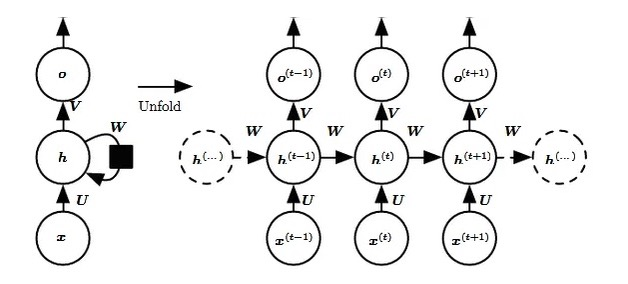
\includegraphics[width=0.8\textwidth]{rnn_diagram.jpeg}
\caption{https://www.deeplearningbook.org/contents/rnn.html}
\end{figure}

However, RNNs have a significant limitation in that they often struggle to learn long term dependencies, since during backpropgation, the gradients are propagated through the same weights matrix multiple times, which especially when dealing with long sequences can lead to the vanishing and exploding gradient problem where the gradients either becomes extremely small or extremely big. Long Short-Term Memory (LSTM) networks  aim to solve this problem. The LSTM network is a modification of the RNN that introduces a second hidden state, called the cell state, which is updated differently from the traditional hidden state. It is governed by these equations:

\begin{equation} a^{(t)} = Wh^{(t-1)} + Ux^{(t)} + b_h\end{equation}

Now $a^{(t)}$ is used to compute four gates, $i$, $f$, $o$, and $g$ with different biases and activation functions:

\begin{equation} i^{(t)} = \sigma(a^{(t)} + b_i) \end{equation}

\begin{equation} f^{(t)} = \sigma(a^{(t)} + b_f) \end{equation}

\begin{equation} o^{(t)} = \sigma(a^{(t)} + b_o) \end{equation}

\begin{equation} g^{(t)} = \tanh(a^{(t)} + b_g) \end{equation}

The gates are used to compute the next cell state, where the $f$ gate decides how much to 'remember' or 'forget' from the previous cell state, and the $i$ and $g$ gate together decide how much new information to write.

\begin{equation} C^{(t)} = f^{(t)} \odot C^{(t-1)} + i^{(t)} \odot g^{(t)} \end{equation}

The $o$ gate then detemines how much of the cell state to output to the next hidden state.

\begin{equation} h^{(t)} = o^{(t)} \odot \tanh(C^{(t)}) \end{equation}

Usually the output vector equals the hidden state in a LSTM.

\begin{equation} y^{(t)} = h^{(t)} \end{equation}

\begin{figure}[h]
\centering
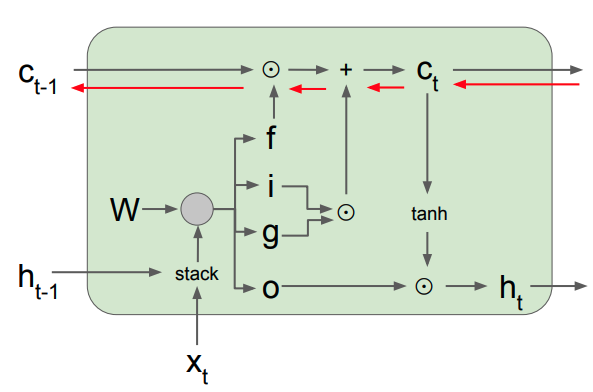
\includegraphics[width=0.6\textwidth]{lstm_diagram.png}
\caption{http://cs231n.stanford.edu/slides/2017/cs231n\_2017\_lecture10.pdf}
\end{figure}

Figure 3 showcases an LSTM cell, notice the red arrows which show the gradient flow. Because the hadamard product is used instead of matrix multiplication and the gates can vary between cells, gradient flow becomes more stable, which allows the network to learn long-term dependencies without an exploding or vanishing gradient.
\subsection{Transformers}

% add this figure somewhere
% \begin{figure}[h]
% \centering
% 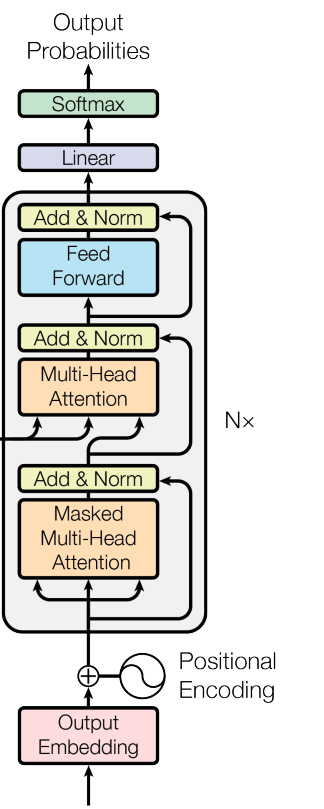
\includegraphics[width=0.2\textwidth]{decoder.png}
% \caption{Transformers decoder architecture, taken from "All you need is attention" by Google. }
% \end{figure}

Transformers is a type of neural network architecture that was introduced in the paper "Attention is all you need" \cite{DBLP:journals/corr/VaswaniSPUJGKP17}. Unlike RNNs, Transformers do not process the data in sequence, instead, they process the entire sequence at once. Transformers transform the data into an embedding layer where the positions are encoded into the data vectors themselves which allows for parallelization.

The key element in Transformers is the self-attention mechanism. In self-attention, each token in the input sequence is transformed with trainable weights into three vectors, a query $Q$, a key $K$ and a value $V$ vector. The query vector represents what a given token is looking for, the key vector what the token offers, whilst the value vector is the information the token contains.

$$\text{Attention}(Q, K , V) = \text{softmax}\left(\frac{QK^T}{\sqrt{d_k}}\right)V$$

The self-attention mechanism takes the dot product between the keys and queries of the tokens, divides it by the square root of the key dimension (to prevent too small gradients) and then applies softmax to create a weights matrix. The weights matrix is used to determine how much each token in the sequence should contribute to the value vector of another token. For example, let the tokens be words in a sentence. In the sentence "The cat sat on the mat", the word "cat" would have a high affinity for the word "mat" (a query vector looking for the object of the sentence) and a low affinity for the word "the". This mechanism allows the network to learn the relationships between the tokens in the sequence. Usually, a specfic form of attention is used, called causal attention or masked attention. In masked attention each output position is only allowed to attend to earlier positions in the input or output sequence, effectively preventing the model from using future information to make its predictions.

The self-attention mechanism is usually applied multiple times on the same tokens in parallel. This is called multi-head attention. For each head $i$, separate trainable transformations are applied to produce new $Q^i$, $K^i$, and $V^i$.

$$\text{head}_i = \text{Attention}(Q^i, K^i, V^i)$$

The results of each head are then concatenated and then linearly transformed to create the final output of the multi-head layer.

$$\text{MultiHead}(Q, K, V) = \text{Concat}(\text{head}_1, \ldots, \text{head}_h)W^O$$

where $W^O$ is also a trainable weight matrix.

\begin{figure}[h]
\centering
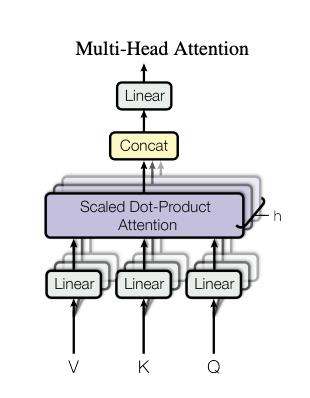
\includegraphics[width=0.3\textwidth]{multi-head.png}
\caption{Taken from "All you need is attention" by Google.}
\end{figure}

The multi-head layer is paired with a position-wise feed-forward layer. The feed-forward layer applies two trainable linear transformations with a ReLU activation in between:

$$\text{FFN}(x) = \text{ReLU}(xW_1 + b_1)W_2 + b_2$$

The feed-forward layer allows the network to learn more complex representations of the data. The multi-head layer and feed-forward layer is usually repeated in blocks to form the transformer network. Between the layers goes a residual connection called layer normalization. Each time a multi-head or a feed-forward layer has made a computation, the result is added to the original input and normalized:

$$\text{LayerNorm}(x + \text{Sublayer}(x))$$

where $\text{Sublayer}(x)$ is the function implemented by the multi-head or feed-forward layer and $x$ is the original input. This residual connection and normalization make the gradient flow more stable through the network.

\subsection{Reservoir Computing and Echo State Networks}

Reservoir Computing (RC) is a variant of RNNs that has proven particularly effective in predicting chaotic systems. The fundamental principle behind reservoir computing is that only a part of the network is trained, while the rest of the network, the "reservoir" remains unchanged during training. This approach significantly reduces the computational cost of training RNNs and overcomes some of the issues related to gradient-based learning in traditional RNNs, such as vanishing and exploding gradients.

Echo State Networks (ESNs) are a particularly well-known implementation of reservoir computing. ESNs consist of a sparsely connected and randomly generated reservoir. The dynamics of the reservoir can be described by:

\begin{equation}
x^{(t)} = \tanh(\mathbf{W}x^{(t-1)} + \mathbf{W_{in}}u^{(t)} + \mathbf{W_{fb}}y^{(t-1)} + b),
\end{equation}

where $x^{(t)}$ is the state vector of the reservoir at time $t$, $u^{(t)}$ is the input vector, $\mathbf{W}$ is the reservoir weight matrix, $\mathbf{W_{in}}$ is the input weight matrix, and $\mathbf{W_{fb}}$ represents connections feeding back previous output. These matrices are randomly generated and not trained. Output is then computed as:

\begin{equation}
y^{(t)} = \mathbf{W_{out}}x{(t)},
\end{equation}

where $y^{(t)}$ is the output vector, and $\mathbf{W_{out}}$ is the output weight matrix, which is trained.

\begin{figure}[h] 
\centering 
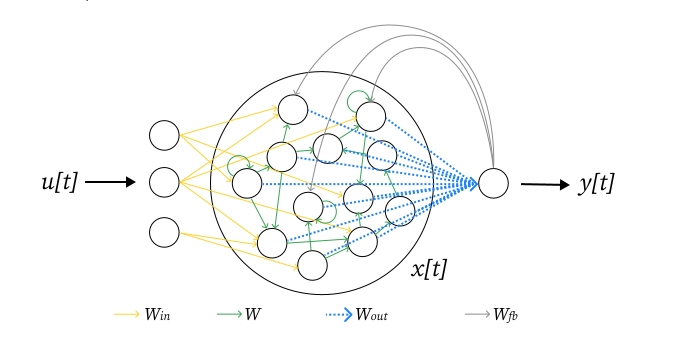
\includegraphics[width=0.8\textwidth]{echo_diagram.png} 
\caption{Echo State Network architecture (image taken from the reservoirpy user guide docs).}
\label{fig:esn}
\end{figure}

The reservoir serves to project the input into a higher-dimensional space where the different parts of the input sequence become more linearly separable. Training only occurs in a readout layer, which is typically a linear model that is adjusted to map the reservoir states to the desired output. Reservoirs in ESNs also possess a "fading memory," enabling them to handle input sequences with varying time scales. This property allows ESNs to maintain the context of earlier inputs while also adapting quickly to recent changes in the input stream.

Training an ESN involves collecting the states of the reservoir for a known input sequence, then using a supervised learning technique, such as linear regression, to determine $\mathbf{W}_{out}$ such that the error between the predicted output $y^{(t)}$ and the actual target output $\hat{y}^{(t)}$ is minimized. This can be expressed as the following optimization problem:

\begin{equation}
\mathbf{W_{out}} = \arg\min_{\mathbf{W_{out}}} \left\{\sum_{t=1}^{n} (\hat{y}^{(t)} - y^{(t)})^2 + \lambda \mathbf{W_{out}}^2\right\},
\end{equation}

Where $n$ is the number of training samples, and $\lambda$ is the regularization parameter that controls the trade-off between fitting the training data and keeping the weights small to avoid overfitting. Notice that this is MSE with an added regularization term.

\section{Method}
The code is written in Python and uses the PyTorch library for implementation of the Transformers and RNN models as well as the ReservoirPy library for the implementation of the ESN. The project is publicly available on GitHub at: \url{https://github.com/SebCodesTheWeb/lorents-net}


\subsection{Generating Data}

The training data is processed via the RK4 method which is implemented in \ref{rk4:lorenz}.

The data is created in the {generate\_dataset.py} module.

\begin{lstlisting}[language=Python]
from lorenz import RK4
import pandas as pd
import numpy as np
from constants import seed_nbr, dt, chunk_len

np.random.seed(seed_nbr)

total_data_points = 1e6
nbr_chunks = int(total_data_points // chunk_len)

pos = [17.67715816276679, 12.931379185960404, 43.91404334248268]

dataset = []
dataset.append({
    't': 0,
    'x': pos[0],
    'y': pos[1],
    'z': pos[2],
})

for i, _ in enumerate(nbr_chunks):
    for j in range(chunk_len):
        elapsedTime = j * dt + dt
        pos = RK4(pos, dt)
        x, y, z = pos
        dataset.append({
            't': elapsedTime,
            'x': x,
            'y': y,
            'z': z
        })
\end{lstlisting}

In this code the constants are $dt = 0.04$, $seed\_nbr = 0$ and $chunk\_len = 10$(100 was used for transformers). These values for $dt$ and $chunk\_len$ have after some trial and error proven effective in generating good data to train the models on. The code generates 1 million datapoints of the Lorenz system with the initial position [17.67715816276679, 12.931379185960404, 43.91404334248268], which was arbitrarily chosen. 

\begin{lstlisting}
dataset = pd.DataFrame(dataset)

dataset.to_csv('lorenz-sequences_raw.csv', index=False)

#Z-score normalization
numerical_cols = ['x', 'y', 'z']
dataset[numerical_cols] = (
    dataset[numerical_cols] - dataset[numerical_cols].mean()

) / dataset[numerical_cols].std()

dataset.to_csv('lorentz-sequences.csv', index=False)
\end{lstlisting}

The dataset is then normalized using Z-score normalization to improve gradient flow, which is critical. The raw unnormalized data is saved in a separate csv file to later on move the model predictions out of normalized space with inverse Z-score normalization \ref{inverse:normalization}.


Afterwards it is split into training, validation and testing sets in the \texttt{get\_training\_data.py} module \ref{datasplit}.

\subsection{Setting up the RNN}

The \texttt{LSTM\_RNN} class defines a RNN network based on PyTorch's \texttt{nn.Module} \ref{lstm}


The model is then instantiated like this:
\begin{lstlisting}
from get_training_data import x_train, y_train
from lstm_rnn import LSTM_RNN
from torch import nn
from torch.utils.data import DataLoader, TensorDataset
import torch.optim as optim
import torch
from torch.optim.lr_scheduler import ExponentialLR
import optuna
from device import device as default_device

def train_rnn_lstm(
    hidden_size=32,
    num_layers=1,
    learning_rate=0.0005,
    batch_size=32,
    epochs=5,
    gamma=0.8,
    trial = None,
    device=default_device,
):
    x_train_device = x_train.to(device)
    y_train_device = y_train.to(device)

    train_data = TensorDataset(x_train_device, y_train_device)
    train_dataloader = DataLoader(train_data, batch_size=batch_size)

    input_size = x_train_device.shape[2]
    output_size = y_train_device.shape[1]
    model = LSTM_RNN(input_size, hidden_size, output_size, num_layers, device).to(device)

    loss_fn = nn.MSELoss()
    optimizer = optim.Adam(model.parameters(), lr=learning_rate)
    scheduler = ExponentialLR(optimizer, gamma=gamma)
\end{lstlisting}

 It uses mean squared error loss function and the adam optimizer. It also uses an exponentially decaying learning step scheduler, which has proven great for managing learning rate with many training epochs. \\ \\  The RNN network is later on iterated over each batch of the training data and the loss is calculated and backpropagated through the network to update the weights. \ref{training:loop}


\subsection{Setting up the Transformers Model}

The transfomers class is written with PyTorch TransformerEncoder and TransformerEncoderLayer classes and is defined in transformer.py \ref{transformer} with positional encoding implemented in the PositionalEncoding class \ref{positional:encoding}.

The model is then trained in a similar fashion to the RNN model and uses the same training loop.

\subsection{Setting up the RC-ESN}

The echo state network was implemented with reservoirpy, a library for reservoir computing in Python in reservoir.py \ref{reservoir}

\subsection{Hyperparameter optimization process}
Firstly a new loss function was defined in true\_loss.py \ref{true:loss} to evaluate the models on unseen data. This was done via generating a new random path with the RK4 method and then comparing the model's predictions to the actual path. The average MSE error was then computed to evaluate the model's performance.


The hyperparameters of the Transformers and RNN networks were then optimized using the optuna library implementation of the Tree-structured Parzen Estimator(TPE) algorithm. 

\begin{lstlisting}
import optuna
import torch
from train_transformer import train_transformer
from train_network import train_rnn_lstm
from true_loss import evaluate_model
import csv
from device import device as default_device

model_type = "Transformer"

def objective(trial):
    learning_rate = trial.suggest_float("learning_rate", 1e-5, 1e-2)
    batch_size = trial.suggest_categorical("batch_size", [4, 8, 16, 32, 64, 128, 256])
    gpu_id = trial.number % 4
    device = torch.device(
        f"cuda:{gpu_id}" if torch.cuda.is_available() else default_device
    )

    if model_type == "Transformer":
        model_hyperparams = {
            "hidden_dim": trial.suggest_categorical(
                "hidden_dim", [256, 512, 768, 1024]
            ),
            "nhead": trial.suggest_int("nhead", 1, 2),
            "num_layers": trial.suggest_int("num_layers", 1, 4),
            "learning_rate": learning_rate,
            "batch_size": batch_size,
            "d_model": trial.suggest_categorical("d_model", [64, 128, 256, 512]),
            "dropout": trial.suggest_float("dropout", 0, 0.4),
            "epochs": 5,
            "trial": trial,
            "device": device,
        }

        model = train_transformer(**model_hyperparams)
        val_loss = evaluate_model(model, device)
        return val_loss

    elif model_type == "RNN_LSTM":
        model_hyperparams = {
            "hidden_size": trial.suggest_categorical(
                "hidden_size", [32, 64, 128, 256, 512]
            ),
            "num_layers": trial.suggest_int("num_layers", 1, 3),
            "learning_rate": learning_rate,
            "batch_size": batch_size,
            "epochs": 5,
            "gamma": trial.suggest_float("gamma", 0.7, 1),
            "trial": trial,
            "device": device,
        }

        model = train_rnn_lstm(**model_hyperparams)
        val_loss = evaluate_model(model, device)
        return val_loss


# Optuna study
pruner = optuna.pruners.MedianPruner()
study = optuna.create_study(
    direction="minimize", pruner=pruner, storage="sqlite:///lorenz_study.db"
)
study.optimize(
    objective, n_trials=100, n_jobs=4, show_progress_bar=True
)  # n_jobs is number of parallel jobs(one per gpu available)
\end{lstlisting}

It was parallelizad to run on four gpus and took use of pruning to preemptively end unpromising trials. Once the best combination of hyperparameters was found the networks was retrained over more epochs for optimal results. The optimization took place over 100 trials and was trained on four RTX 4090s.

The ESN was on the hand manually optimized by trial and error, as the reservoirpy library does not support optuna.

In the end the following hyperparameters were used in the final models:

\begin{itemize}
    \item \textbf{ESN:}
    \begin{itemize}
        \item reservoir size: 1000
        \item leakage rate: 0.5
        \item spectral radius: 0.9
        \item ridge parameter: $2.5 \times 10^{-6}$
        \item inp\_seq\_len: 1
    \end{itemize}
    \item \textbf{Transformers:}
    \begin{itemize}
        \item hidden\_dim: 256
        \item nhead: 2
        \item num\_layers: 2
        \item learning\_rate: 0.002569758352546269
        \item batch\_size: 64
        \item d\_model: 64
        \item dropout: 0.020779607365612865
        \item epochs: 30
        \item inp\_seq\_len: 49
    \end{itemize}
    \item \textbf{RNN LSTM:}
    \begin{itemize}
        \item hidden\_size: 32
        \item num\_layers: 1
        \item learning\_rate: 0.0005
        \item batch\_size: 32
        \item epochs: 10
        \item gamma: 8
        \item inp\_seq\_len: 9
    \end{itemize}
\end{itemize}

The models were then finally evaluated by predicting 500 time steps and comparing the predictions to the testing data set. To evaluate the models, their Lorenz attractor shape, trajectory and mean squared error was plotted.

\section{Results}
\subsection{Lorenz attractor}
\begin{figure}[ht]
    \centering
    \begin{minipage}{0.32\textwidth}
        \centering
        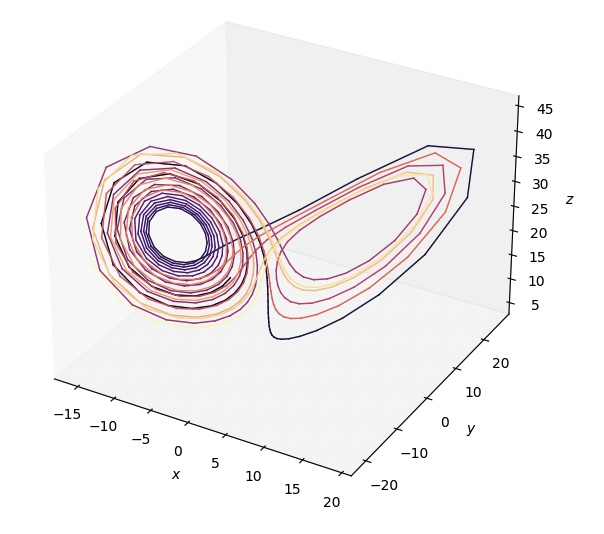
\includegraphics[width=\textwidth]{rnn_lorenz.jpeg}
        \caption{RNN}
    \end{minipage}\hfill
    \begin{minipage}{0.32\textwidth}
        \centering
        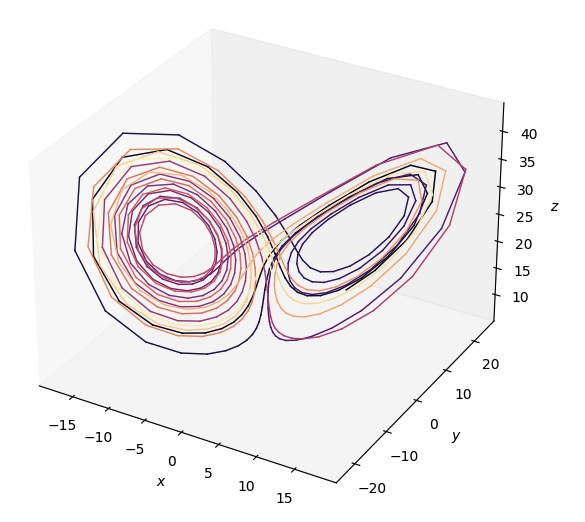
\includegraphics[width=\textwidth]{echo_lorenz.jpeg}
        \caption{ESN}
    \end{minipage}\hfill
    \begin{minipage}{0.32\textwidth}
        \centering
        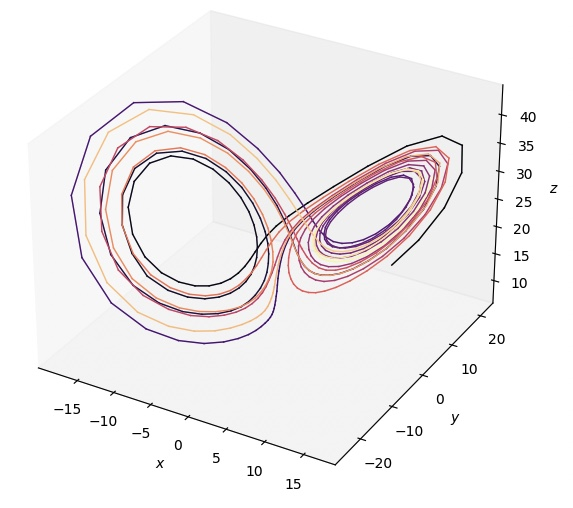
\includegraphics[width=\textwidth]{transformers_lorenz.jpeg}
        \caption{Transformers}
    \end{minipage}
\end{figure}

\subsection{Trajectory}
View figures 10, 11 and 12.

\begin{figure}[p]
    \centering
    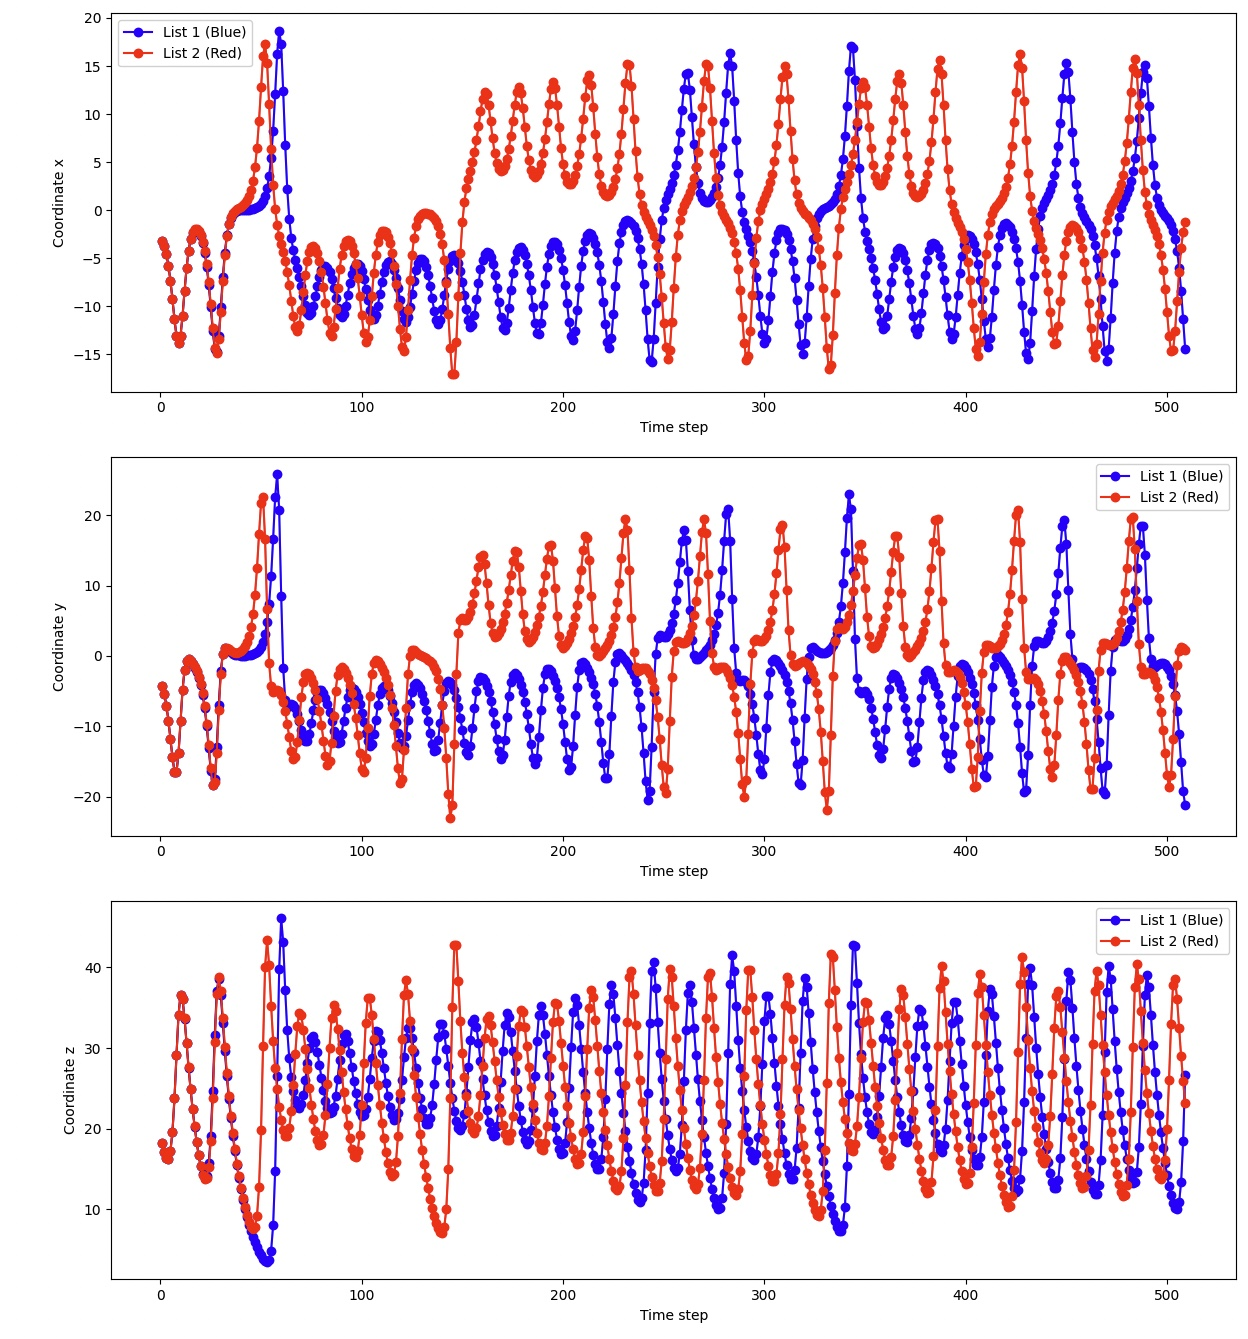
\includegraphics[width=\textwidth]{rnn_path.jpeg}
    \caption{RNN path(true path is red, model path is blue)}
\end{figure}

\begin{figure}[p]
    \centering
    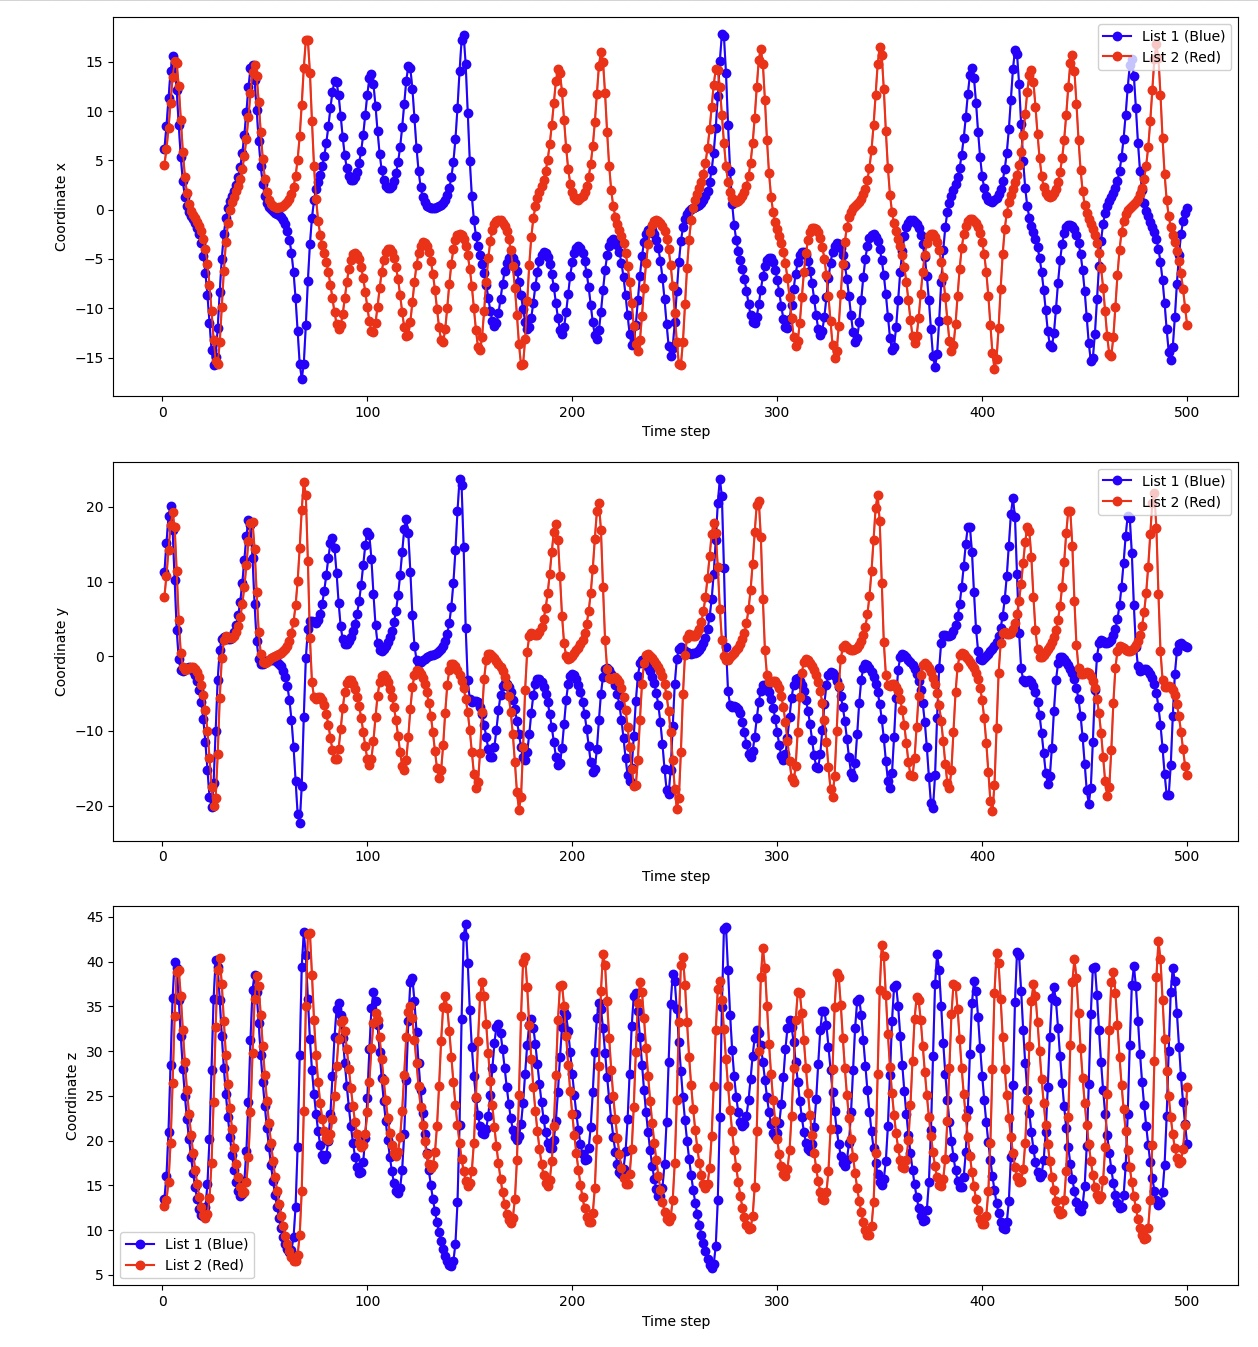
\includegraphics[width=\textwidth]{echo_path.jpeg}
    \caption{ESN path(true path is red, model path is blue)}
\end{figure}

\begin{figure}[p]
    \centering
    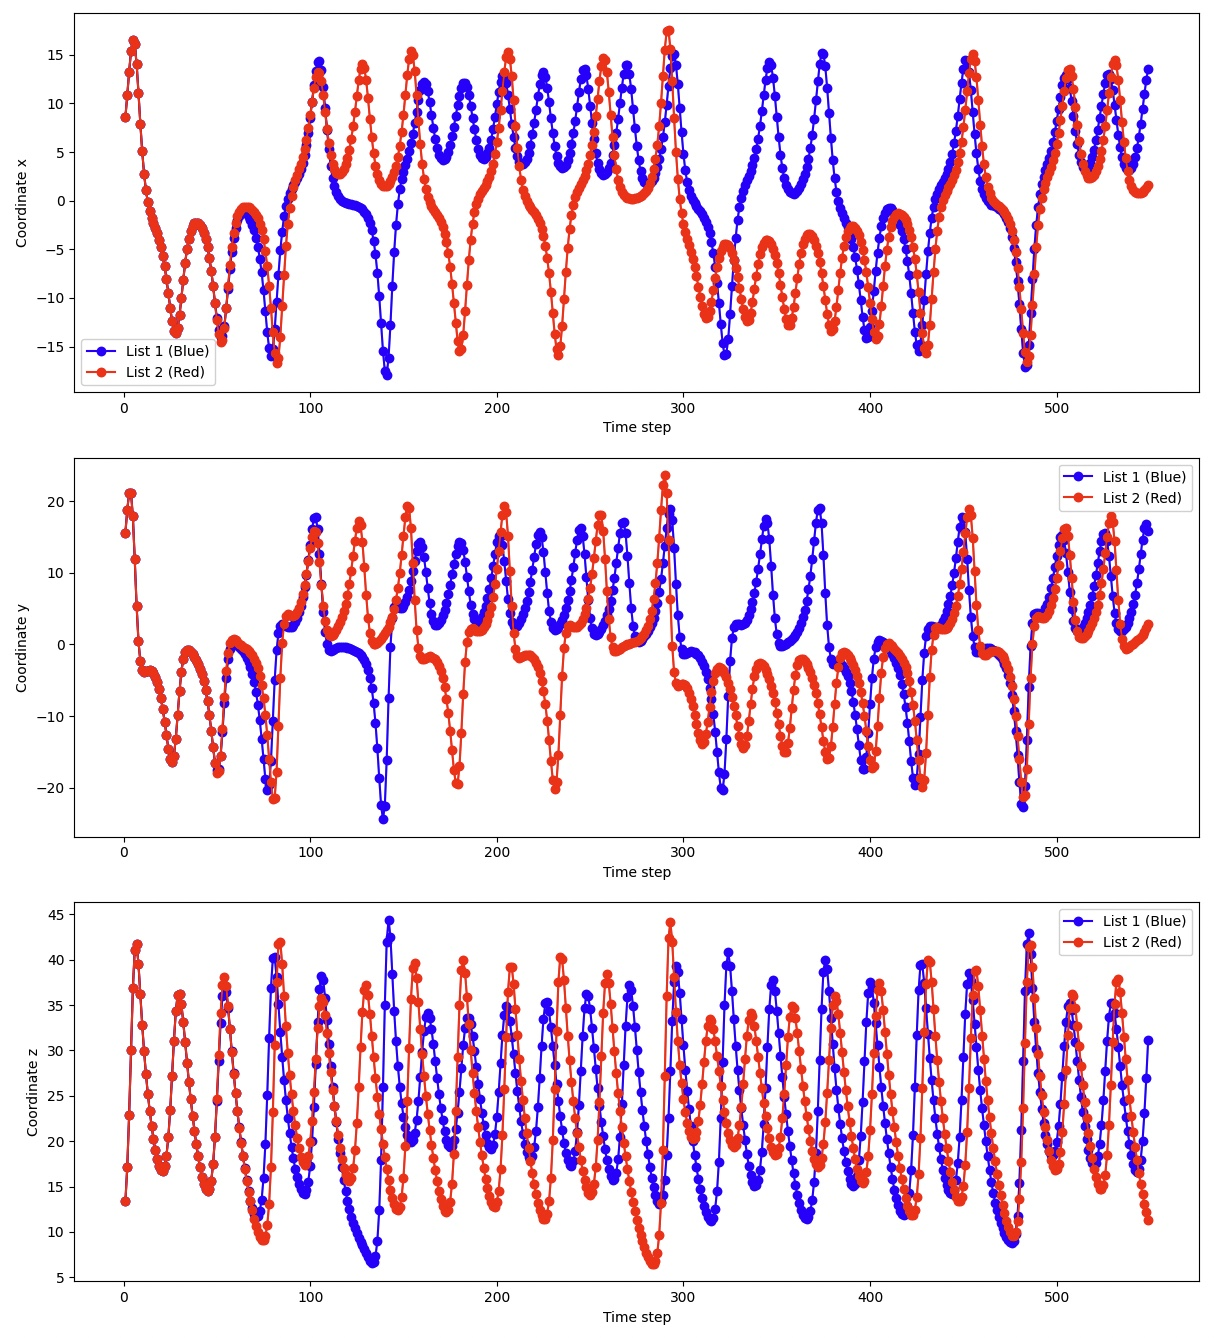
\includegraphics[width=\textwidth]{transformers_path.jpeg}
    \caption{Transformers path(true path is red, model path is blue)}
\end{figure}

\subsection{Mean Squared Error}
\begin{figure}[h]
\centering
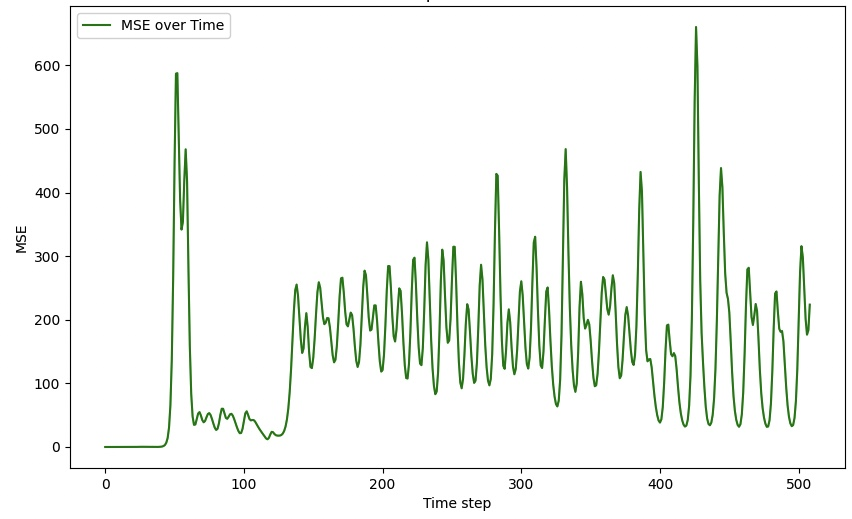
\includegraphics[width=0.6\textwidth]{rnn_mse.jpeg}
\caption{RNN MSE}
\end{figure}

\begin{figure}[h]
\centering
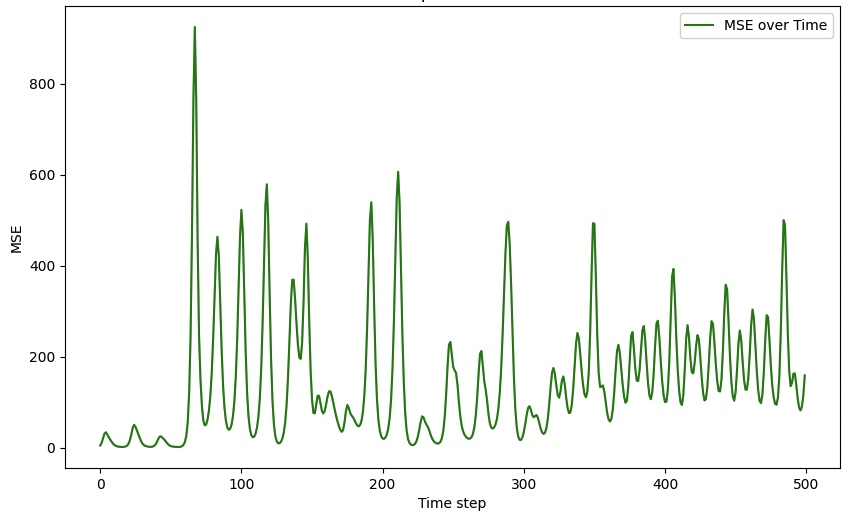
\includegraphics[width=0.6\textwidth]{echo_mse.jpeg}
\caption{ESN MSE}
\end{figure}

\begin{figure}[h]
\centering
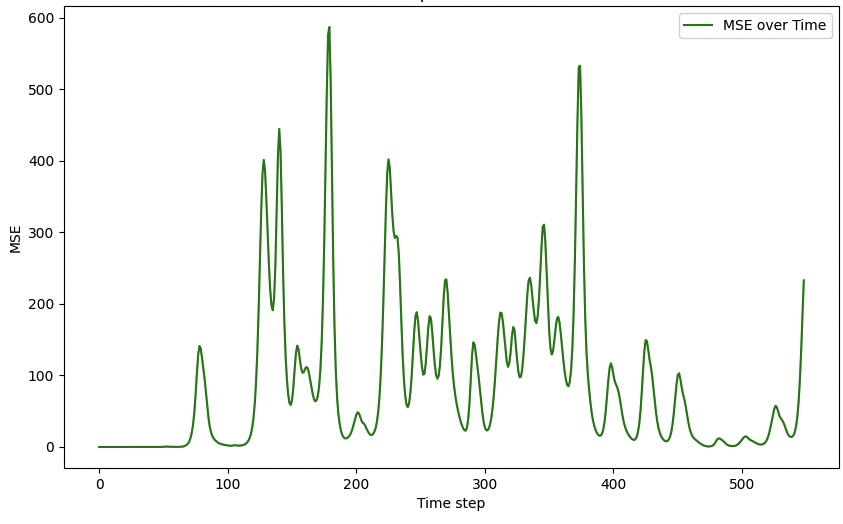
\includegraphics[width=0.6\textwidth]{transformers_mse.jpeg}
\caption{Transformers MSE}
\end{figure}
The average MSE for RNN was 50.1579 \\
The average MSE for RNN was 48.7797 \\
The average MSE for RNN was 29.1590 \\ \\
For a more detailed overview of MSE over time view figures 13, 14 and 15.

\section{Discussion}
Looking at figures 7-9, it is clear that all models have learned the Lorenz patterns, thereby the underlying dynamics of the system. They all generated attractors of similar scale with two rings centering around two focal points. They differ slightly, however, and when comparing the figures, it is hard to tell which of the models has captured the best attractor shape (see figure 1). The Transformers model seems to have the most accurate angle between the two rings, but the left wing radius should be smaller and the outer right wing radius should be bigger. The ESN has more accurate outer wing radii, but the RNN seems to have more accurate inner wing radii. Overall, however, it seems like the ESN network has the most accurate Lorenz attractor shape.

The results from the trajectory plots are clear. In figure 10, the RNN path seems to deviate from the true path around timestep 40-50, which is confirmed by figure 13 where the MSE could be seen spiking. The MSE then goes down for a bit, showing that the RNN has learned the pattern of the Lorenz attractor but not with great accuracy.

Viewing figure 11, the ESN seems to diverge from the true path around timestep 60-100, which also is confirmed by figure 14 showcasing some big up and down spikes. The MSE seems to vary a lot, which shows that the ESN has not learned the Lorenz system's trajectory very accurately, but has learned the overall pattern and can follow it for a while.

Looking at figure 12, the Transformers model seems to follow the true path very well up till timestep 100-120. This is confirmed by figure 15 where the MSE is very low and stable untill slightly after timestep 100. The Transformers model also appears to hop back on track around timestep 400 and follow the true path accurately for another 100 timesteps.

Keeping in mind that the ESN has a $inp\_seq\_len$ of 1, the RNN a $inp\_seq\_len$ of 9, and the Transformers model a $inp\_seq\_len$ of 49, the ESN could hold an accurate prediction for about 70-80 timesteps. The RNN could hold an accurate prediction for about 30-40 timesteps. And the Transformers model could hold an accurate prediction for about 60 timesteps with a small bounce back where it held a good prediction for about another 100 more timesteps. Overall, the Transformers model had the lowest MSE.

\subsection{Conclusion}
The results are a bit mixed but it seems clear that the RNN was the worst performing model. It had the highest MSE, could hold a prediction for only 30-40 timesteps and did not have a very impressive Lorenz attractor. The ESN had an accurate Lorenz attractor and could hold the initial prediction the longest, but the Transformers model had much lower MSE without much shorter initial prediction accuracy. The difference does not seem significant enough to make a data-driven conclusion, but seeing as less efforts was spent optimizing the ESN model and it has in other literature shown great capabilities in predicting chaotic systems \cite{npg-27-373-2020}, it seems reasonable to assume the ESN has a slight edge over the Transformers model, although a small one. Hence the results of this study show that the ESN seems to be the best neural network architecture for predicting chaotic systems, tightly followed by the Transformers model and RNN last.

The results show that the Transformers architecture has an impressive capacity to capture chaotic dynamics, similar to the level of an ESN, whilst the RNN is not as well suited towards capturing chaotic dynamics. For future research the NVAR reservoir computing variant could be explored, as it in other literature(\cite{cite-key}) has shown great promise. Other hyperparameters of the ESN such as noise could be explored for further optimization, which was not attempted in this study. Regarding the Transformers architecture, different positional embeddings could be used, and the variations of the self attention mechanism like sparse attention could be investigated. With further research it may be possible to conclusively state the peak potential of the Transformers and ESN models in predicting chaotic systems.


\clearpage

\appendix
\section*{Appendix}
\section{Code snippets}
\label{appendix:code}

\begin{lstlisting}[label=rk4:lorenz, caption={RK4 implementation}]
import numpy as np

sigma =  10
rho = 28
beta = 8/3

def get_derivative(pos_vector):
    x, y, z = pos_vector

    dx_dt = sigma*(y-x)
    dy_dt = x*(rho-z)-y
    dz_dt = x*y - beta*z

    return np.array([dx_dt, dy_dt, dz_dt])

def RK4(pos_vector, dt):
    k1 = dt * get_derivative(pos_vector)
    k2 = dt * get_derivative(pos_vector + k1/2)
    k3 = dt * get_derivative(pos_vector+ k2/2)
    k4 = dt * get_derivative(pos_vector + k3)

    return pos_vector + (k1 + 2*k2 + 2*k3 + k4) / 6

\end{lstlisting}

\begin{lstlisting}[label=datasplit, caption={get\_training\_data.py}]
import pandas as pd
import torch
import numpy as np
from constants import (
    inp_seq_len,
    val_ratio,
    seed_nbr,
)

dataset = pd.read_csv("lorentz-sequences.csv")
data_tensor = torch.tensor(dataset[["x", "y", "z"]].values, dtype=torch.float32)

test_set = data_tensor[-10000:].numpy().tolist()
data_tensor = data_tensor[:-10000]


def create_seq(data):
    seq = []
    for i in range(0, len(data) - inp_seq_len, inp_seq_len):
        input = data[i : i + inp_seq_len]
        label = data[i + inp_seq_len]
        # Given input sequence, predict the next value(label)
        seq.append((input, label))
    return seq


data_seq = create_seq(data_tensor)


def manual_split(data, val_ratio, seed):
    np.random.seed(seed)
    num_examples = len(data)
    val_size = int(num_examples * val_ratio)

    shuffled_indices = np.random.permutation(num_examples)
    val_indices = shuffled_indices[:val_size]
    train_indices = shuffled_indices[val_size:]

    train_data = [data[i] for i in train_indices]
    val_data = [data[i] for i in val_indices]

    return train_data, val_data


inout_seq_train, inout_seq_val = manual_split(data_seq, val_ratio, seed_nbr)

# item[0] is input sequence, item[1] is label
x_train = torch.stack([item[0] for item in inout_seq_train])
y_train = torch.stack([item[1] for item in inout_seq_train])
x_val = torch.stack([item[0] for item in inout_seq_val])
y_val = torch.stack([item[1] for item in inout_seq_val])

\end{lstlisting}

The function splits the training data into a list of separate, trainable sequences, where each individual sequence has a label(the next value to predict) associated with it. These data sequences are later split into a training and validation sets with a 85/15 ratio. The validation set will be used to optimize the hyperparameters of the models. Notice also that the last 10000 data points were split off for a final testing set.

\begin{lstlisting}[label=lstm, caption={LSTM RNN implementation}]
import torch
import torch.nn as nn
from device import device as default_device

class LSTM_RNN(nn.Module):
    def __init__(self, input_size, hidden_size, output_size, num_layers=1, device=default_device):
        """
        input_size: input feature size, in this case 3 for the Lorenz system
        output_size: output feature size, in this case 3 for the Lorenz system
        hidden_size: number of hidden units in the LSTM
        """
        super(LSTM_RNN, self).__init__()
        self.hidden_size = hidden_size
        self.num_layers = num_layers

        self.lstm = nn.LSTM(
            input_size, hidden_size, num_layers=num_layers, batch_first=True
        )
        self.output_activation = nn.Linear(hidden_size, output_size)
        self.device = device

    def forward(self, inputSeq):
        # inputSeq shape [batch_size, seq_len, feature_size]
        batch_size = inputSeq.size(0)
        state = self.init_state(batch_size)
        lstm_out, _ = self.lstm(inputSeq, state)

        # Select the last point in the sequence
        prediction = self.output_activation(lstm_out[:, -1, :])

        return prediction

    def init_state(self, batch_size):
        # Initializing the hidden and cell states for the LSTM based on the batch size
        state = (
            torch.zeros(self.num_layers, batch_size, self.hidden_size).to(self.device),
            torch.zeros(self.num_layers, batch_size, self.hidden_size).to(self.device),
        )
        return state
\end{lstlisting}

\texttt{input\_size} is the dimensionality of the input vector(in this case three for the x, y and z values). The constructor initializes the LSTM layer and output activation layer. The \texttt{forward} method is passing the input through the torhc.nn.LSTM cell and the activation layer to compute the output. The \texttt{init\_state} method initializes the LSTM's internal state with zeros for each new batch. \\

\begin{lstlisting}[caption={inverse normalization}, label=inverse:normalization]
import pandas as pd

dataset = pd.read_csv("lorenz-sequences_raw.csv")

mean_x, std_x = dataset["x"].mean(), dataset["x"].std()
mean_y, std_y = dataset["y"].mean(), dataset["y"].std()
mean_z, std_z = dataset["z"].mean(), dataset["z"].std()


def get_unnormalized_prediction(predictions: list):
    unnormalized_predictions = [
        [(x * std_x) + mean_x, (y * std_y) + mean_y, (z * std_z) + mean_z]
        for x, y, z in predictions
    ]

    return unnormalized_predictions
\end{lstlisting}

\begin{lstlisting}[caption={Training loop}, label=training:loop]
def train(dataloader, model, loss_fn, optimizer):
    size = len(dataloader.dataset)
    num_batches = len(dataloader)
    model.train()
    running_loss = 0.0

    for batch_nbr, (seq, label) in enumerate(dataloader):
        seq, label = seq.to(device), label.to(device)
        label = label.squeeze(1) # Remove the extra middle dimension, in this case label shape is [batch_size, 1, feature_size]
        prediction = model(seq)
        loss = loss_fn(prediction, label)

        optimizer.zero_grad()
        loss.backward()
        optimizer.step()

        running_loss += loss.item()
        if batch_nbr % 100 == 0:
            current = batch_nbr * len(seq)
            print(f"loss: {loss:>7f}  [{current:>5d}/{size:>5d}]")

    running_loss /= num_batches
    print(f"Average loss for epoch: {running_loss:>7f}")
    return running_loss

for t in range(epochs):
    print(f"epoch {t + 1} \n--------------")
    train(train_dataloader, model, loss_fn, optimizer)
    if trial is not None:
        trial.report(loss, t)
        if trial.should_prune():
            raise optuna.exceptions.TrialPruned()

    scheduler.step()
print("Done")
torch.save(model.state_dict(), 'lstm_rnn_lorenz.path')
\end{lstlisting}
The training loop iterates over the dataset, feeding batches of data to the model, calculating the loss, and updating the model parameters through backpropagation. Finally after five epochs, the model's parameters are saved.

\begin{lstlisting}[caption={Transformer implementation}, label=transformer]
import math
import torch
from torch import nn, Tensor
from torch.nn import TransformerEncoder, TransformerEncoderLayer

class TransformerModel(nn.Module):
    def __init__(self, ntoken: int, d_model: int, nhead: int, d_hid: int, nlayers: int, dropout: float = 0.5):
        """
        ntoken: The size of the vocabulary (total number of unique tokens).
        d_model: The dimensionality of the token embeddings (the size of the vectors that represent each token).
        nhead: The number of attention heads in the multi-head attention mechanisms.
        d_hid: The dimensionality of the feedforward network model in the transformer encoder.
        nlayers: The number of sub-encoder-layers in the transformer encoder.
        dropout: The dropout rate, a regularization technique to prevent overfitting.


        """
        super().__init__()
        self.model_type = 'Transformer'
        self.pos_encoder = PositionalEncoding(d_model, dropout)
        encoder_layers = TransformerEncoderLayer(d_model, nhead, d_hid, dropout, batch_first=True)
        self.transformer_encoder = TransformerEncoder(encoder_layers, nlayers)
        ##Use linear layer instead of traidiontal embedding layer due to continous data
        self.input_linear = nn.Linear(3, d_model)
        self.d_model = d_model
        self.output_linear = nn.Linear(d_model, 3)

        self.init_weights()

    def init_weights(self) -> None:
        initrange = 0.1
        self.input_linear.weight.data.uniform_(-initrange, initrange)
        self.input_linear.bias.data.zero_()
        self.output_linear.bias.data.zero_()
        self.output_linear.weight.data.uniform_(-initrange, initrange)

    def forward(self, src: Tensor) -> Tensor:
        """
        Arguments:
            src: Tensor, shape ``[seq_len, batch_size]``
            src_mask: Tensor, shape ``[seq_len, seq_len]``

        Returns:
            output Tensor of shape ``[seq_len, batch_size, ntoken]``
        """
        src = self.input_linear(src) * math.sqrt(self.d_model)
        src = self.pos_encoder(src)
        output = self.transformer_encoder(src)
        output = self.output_linear(output)
        return output
    
\end{lstlisting}

The input is first passed through a linear layer to transform the input data into the d\_model dimensionality. The input is then passed through a positional encoding layer to add information about the position of the tokens in the sequence. The output is then passed through the transformer encoder and then through a linear layer to transform the output back to the original dimensionality. The positional encoding is defined as:

\begin{lstlisting}[caption={Positional encoding implementation}, label=positional:encoding]
class PositionalEncoding(nn.Module):
    def __init__(self, d_model: int, dropout: float = 0.1, max_len: int = 5000):
        super().__init__()
        self.dropout = nn.Dropout(p=dropout)

        position = torch.arange(max_len).unsqueeze(1)
        div_term = torch.exp(torch.arange(0, d_model, 2) * (-math.log(10000.0) / d_model))
        pe = torch.zeros(max_len, 1, d_model)
        pe[:, 0, 0::2] = torch.sin(position * div_term)
        pe[:, 0, 1::2] = torch.cos(position * div_term)
        self.register_buffer('pe', pe)

    def forward(self, x) :
        """
        Arguments:
            x: Tensor, shape ``[seq_len, batch_size, embedding_dim]``
        """
        x = x + self.pe[:x.size(0)]
        return self.dropout(x)
\end{lstlisting}

The PositionalEncoding module in this code leverages sine and cosine functions to generate a sequence of positional encoding vectors up a maximum length of 5000. Even indices are used with sine and odd indices with cosine to give each vector a unique sequence position. Upon forward pass the positional encoding are added to the input vectors and then passed through a dropout layer to prevent overfitting.  

\begin{lstlisting}[caption={ESN implementation}, label=reservoir]
import reservoirpy as rpy
from constants import seed_nbr, dt
from reservoirpy.nodes import Reservoir, Ridge
import matplotlib.pyplot as plt
import numpy as np
from unnormalize_data import get_unnormalized_prediction
import json
import pandas as pd

rpy.verbosity(999)
rpy.set_seed(seed_nbr)

train_time = 10.
test_time = 20.
warm_time = 5.

train_steps = round(train_time / dt)
test_steps  = round(test_time  / dt)
warm_steps  = round(warm_time  / dt)

n_timesteps = train_steps + test_steps + warm_steps

dataset = pd.read_csv("lorentz-sequences.csv")
X = dataset[["x", "y", "z"]].values

reservoir = Reservoir(1000,  lr=0.5, sr=0.9)
readout = Ridge(3, ridge=2.5e-6)
esn_model = reservoir >> readout

X_train = X[:train_steps + warm_steps -1]
Y_train = X[1:train_steps + warm_steps] - X[:train_steps + warm_steps -1]

model = esn_model.fit(X_train, Y_train, warmup=warm_steps)
    
\end{lstlisting}

The ESN is structured with a Reservoir node and a Ridge regression readout, connected sequentially to construct the model. Training data is prepared by segmenting the input array and generating target output through shifting forward by one step(in this case $inp\_seq\_len$ is 1). Lastly, the model fitting process is carried out, adjusting output weights matrix.


\begin{lstlisting}[caption={true\_loss.py}, label=true:loss]
import numpy as np
import torch
from constants import inp_seq_len, dt, seed_nbr
from lorenz import RK4
from mse import calculate_aggregate_mse
from unnormalize_data import get_unnormalized_prediction
from device import device as default_device

np.random.seed(seed_nbr)


def validate_long_term(nbrIter, init_input_seq, model, device):
    predicted_path = [*init_input_seq]
    for _ in range(nbrIter):
        input_seq = np.array(predicted_path[-inp_seq_len:])
        input_seq_tensor = (
            torch.tensor(input_seq, dtype=torch.float32).unsqueeze(0).to(device)
        )
        with torch.no_grad():
            next_pos = model(input_seq_tensor)

        next_pos = next_pos.cpu().numpy().reshape(-1)
        predicted_path.append(next_pos)

    true_path = [*init_input_seq]
    for _ in range(nbrIter):
        true_path.append(RK4(np.array(true_path[-1]), dt).tolist())

    unnormalized_path = true_path[:inp_seq_len] + get_unnormalized_prediction(
        predicted_path[inp_seq_len:]
    )

    total = 0
    for i in range(3):
        list_a = [x[i] for x in true_path[inp_seq_len:]]
        list_b = [x[i] for x in unnormalized_path[inp_seq_len:]]
        mse_loss_ag = calculate_aggregate_mse(list_a, list_b)
        total += mse_loss_ag
    total /= 3

    return total


init_seq = [np.random.rand(3)]
for _ in range(inp_seq_len - 1):
    next_pos = RK4(np.array(init_seq[-1]), dt)
    init_seq.append(next_pos.tolist())


def evaluate_model(model, device=default_device):
    loss = validate_long_term(
        1000,
        init_seq,
        model,
        device,
    )
    print(f"Validation loss: {loss}")
    return loss
\end{lstlisting}

\bibliographystyle{apalike}
\bibliography{references}

\end{document}

\end{document}
